\documentclass[12pt]{article}

\usepackage[a4paper, margin=1in]{geometry}
\usepackage{fancyhdr}
\usepackage{titling}
\usepackage[latvian]{babel}
\usepackage{graphicx}
\usepackage{float}
\usepackage{dirtytalk}
\usepackage{gensymb}
\usepackage[utf8]{inputenc}
\usepackage[T1]{fontenc} 
\usepackage{amsmath}
\usepackage{hyperref}
\usepackage{listings}
\usepackage{titling}

\newlength\tindent
\setlength{\tindent}{\parindent}
\setlength{\parindent}{0pt}
\renewcommand{\indent}{\hspace*{\tindent}}

\fancypagestyle{plain}{
  \fancyhf{}
  \fancyhead[R]{ Andrejs Cvečkovskis \\ ac24005 \\ Kurss \say{Zinātniskā programmēšana fiziķiem}}
  \renewcommand{\headrulewidth}{0pt}
}

\title{%
  \centering                              % centre the whole block
  Laboratorijas darbs\\[1ex]              % main line
  \large ``Monte--Karlo metode''}          % subtitle in quotes
\author{}
\date{}  
\begin{document} 
\maketitle
\vspace*{-6em}

1. Attēls ar izmestajām šautriņām riņķī

\textbf{Atbilde:}

\begin{center}
    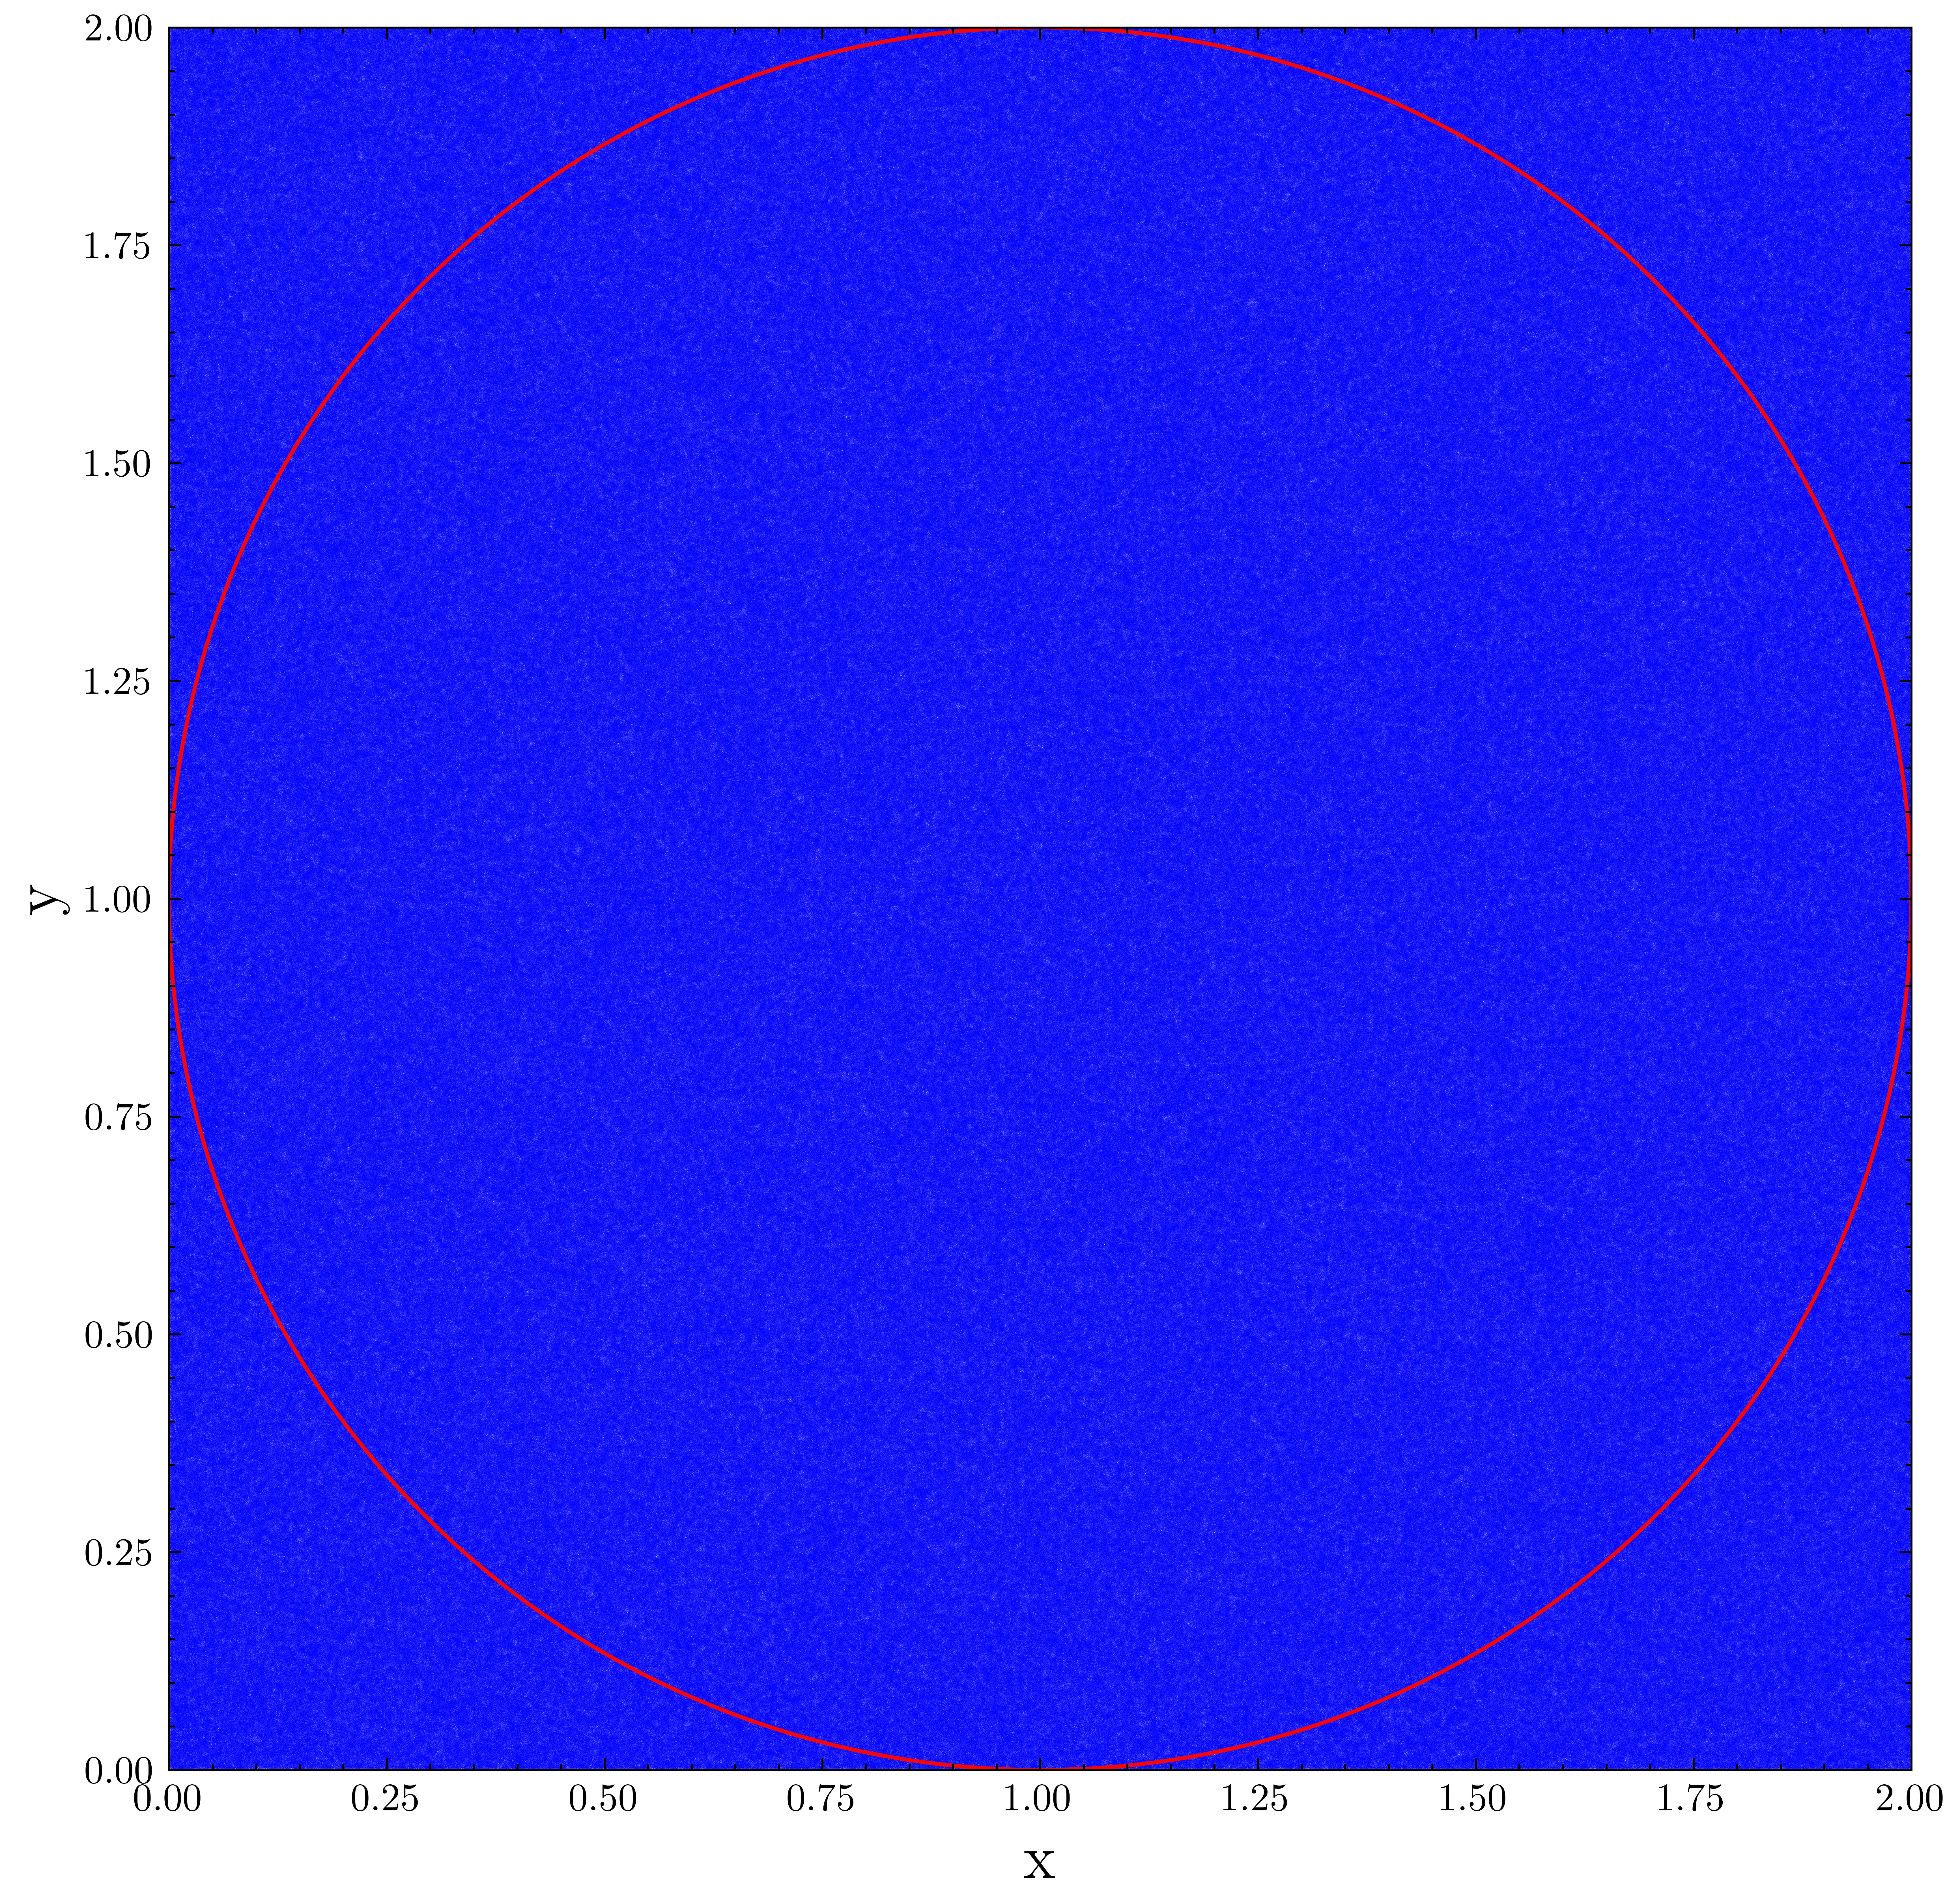
\includegraphics[width=0.8\linewidth]{pi_circle_estimate.png}
\end{center} \\

2. Iegūta $\pi$ aproksimācija

\textbf{Atbilde:} $\pi \approx 3.141618$ \\

3. Kods šautriņu mešanai pa riņķi

\begin{lstlisting}[language=Python]
n = 10000000

x = np.random.uniform(0, 2, n)
y = np.random.uniform(0, 2, n)

inside = (x - 1)**2 + (y - 1)**2 <= 1

count_inside = np.sum(inside)

pi_estimate = 4 * count_inside / n
print(r"Estimated value of $\pi$:", pi_estimate)

fig, ax = plt.subplots(figsize=(8, 8))
ax.scatter(x, y, s=0.0001, color='blue')
circle = plt.Circle((1, 1), 1, color='red', fill=False)
ax.add_artist(circle)
ax.set_aspect('equal', adjustable='box')
ax.set_xlim(0, 2)
ax.set_ylim(0, 2)
ax.set_xlabel('x', fontsize=16)
ax.set_ylabel('y', fontsize=16)
plt.savefig(os.path.join(path, 'pi_circle_estimate'), dpi=1000, 
bbox_inches='tight')
plt.show()
\end{lstlisting}\\

4. Attēls ar izmestajām šautriņām sarežģītajā figūrā

\textbf{Atbilde:} 

\begin{center}
    \includegraphics[width=0.8\linewidth]{monte_carlo_area_estimate.png}
\end{center}
\\

5. Iegūtā sarežģītās figūras laukuma aproksimācija

\textbf{Atbilde:} $S = 9.812352 \hspace{0.1cm}(l.v.)$ \\

6. Kods šautriņu mešanai pa sarežģīto figūru

\begin{lstlisting}
def func(x, y):
    return x**2 + 2*x*y + y**4 < 3

def monte_carlo(func, bounds, n=1000000):
    x_min, x_max, y_min, y_max = bounds
    x_rand = np.random.uniform(x_min, x_max, n)
    y_rand = np.random.uniform(y_min, y_max, n)
    
    inside = func(x_rand, y_rand)
    count_inside = np.sum(inside)
    area_rectangle = (x_max - x_min) * (y_max - y_min)
    area_inside = area_rectangle * count_inside / n
    return x_rand, y_rand, inside, area_inside

bounds = (-3, 3, -2, 2)
n_points = 1000000

x_rand, y_rand, inside, area_estimate = monte_carlo(func,
bounds, n_points)
print("Estimated area under the curve:", area_estimate)

fig, ax = plt.subplots(figsize=(8, 8))
ax.scatter(x_rand[inside], y_rand[inside], s=1, color="green",
label="Inside points")
ax.scatter(x_rand[~inside], y_rand[~inside], s=1, color="red",
label="Outside points")

x = np.linspace(bounds[0], bounds[1], 400)
y = np.linspace(bounds[2], bounds[3], 400)
X, Y = np.meshgrid(x, y)
Z = X**2 + 2*X*Y + Y**4

ax.contourf(X, Y, Z, levels=[-1e10, 3], colors=['lightgreen'], alpha=0.5)
ax.contour(X, Y, Z, levels=[3], colors='black', linewidths=2)
ax.axhline(0, color='black', lw=0.5, ls='--')
ax.axvline(0, color='black', lw=0.5, ls='--')
ax.set_xlabel('x', fontsize=16)
ax.set_ylabel('y', fontsize=16)
plt.savefig(os.path.join(path, 'monte_carlo_area_estimate'), dpi=1000, 
bbox_inches='tight')
plt.show()
\end{lstlisting}

7. Vidējais gājienu skaits un nepieciešamā gājienu skaita histogramma Cirkam bez lēcieniem

\textbf{Atbilde:} 34.4535

\begin{center}
    \includegraphics[width=0.8\linewidth]{throws_needed_histogram.png}
\end{center}

\\

8. Kods Cirkam bez lēcieniem

\begin{lstlisting}[language=Python]
n = 10000
target = 119
throws_needed = np.zeros(n, dtype=int)

for i in range(n):
    total = 0
    throws = 0
    while total < target:
        total += np.random.randint(1, 7) 
        throws += 1
    throws_needed[i] = throws

avg_throws = np.mean(throws_needed)
print("Average number of throws:", avg_throws)

plt.figure(figsize=(8, 8))
plt.hist(throws_needed, bins=range(throws_needed.min(), throws_needed.max()+2),
edgecolor='black')
plt.xlabel('Gājienu skaits')
plt.ylabel('Biežums')
plt.savefig(os.path.join(path, 'throws_needed_histogram'), dpi=1000,
bbox_inches='tight')
plt.show()
\end{lstlisting}

9. Vidējais gājienu skaits un nepieciešamā gājienu skaita histogramma Cirkam ar lēcieniem

\textbf{Atbilde:} 48.0615

\begin{center}
    \includegraphics[width=0.8\linewidth]{throws_needed_leaps_histogram.png}
\end{center}

\\

10. Kods Cirkam ar lēcieniem

\begin{lstlisting}[language=Python]
n = 10000
throws_needed = np.zeros(n, dtype=int)
for i in range(n):
    pos = 1
    throws = 0
    while pos < 120:
        roll = np.random.randint(1, 7)
        # if the dice roll is enough to finish the game:
        if pos + roll >= 120:
            throws += 1
            pos += roll
            break
        else:
            pos += roll
            # check if the new position is a leap start:
            idx = np.where(no == pos)[0]
            if idx.size > 0:
                pos = int(uz[idx[0]])
            throws += 1
    throws_needed[i] = throws

avg_throws = np.mean(throws_needed)
print("Average number of throws with leaps:", avg_throws)

plt.figure(figsize=(8, 8))
plt.hist(throws_needed, bins=range(throws_needed.min(), throws_needed.max()+2),
edgecolor='black')
plt.xlabel('Gājienu skaits')
plt.ylabel("Biežums")
plt.savefig(os.path.join(path, 'throws_needed_leaps_histogram'), dpi=1000,
bbox_inches='tight')
plt.show()
\end{lstlisting}

11. Vidējais gājienu skaits un nepieciešamā gājienu skaita histogramma Cirkam ar lēcieniem un gaidīšanas noteikumu

\textbf{Atbilde:} 67.4623

\begin{center}
    \includegraphics[width=0.8\linewidth]{throws_needed_waiting_histogram.png}
\end{center}

\\

12. Kods Cirkam ar lēcieniem un gaidīšanas noteikumu

\begin{lstlisting}[language=Python]
n = 10000
throws_needed = np.zeros(n, dtype=int)

for i in range(n):
    pos = 1
    throws = 0
    while pos < 120:
        roll = np.random.randint(1, 7)
        
# apply waiting rule: if the roll would overshoot 120, 
# count the turn and skip moving
        if pos + roll > 120:
            throws += 1
            continue
        elif pos + roll == 120:
# exact finish roll: update position and finish game
            throws += 1
            pos = 120
            break
        else:
# normal move: update position and count turn
            pos += roll
            throws += 1
            
# check for leap rule: if landed on a leap start, update position
            idx = np.where(no == pos)[0]
            if idx.size > 0:
                pos = int(uz[idx[0]])
                
    throws_needed[i] = throws

avg_throws = np.mean(throws_needed)
print("Average number of throws with waiting rule:", avg_throws)

plt.figure(figsize=(8, 8))
plt.hist(throws_needed, bins=range(throws_needed.min(), throws_needed.max()+2),
edgecolor='black')
plt.xlabel("Gājienu skaits")
plt.ylabel("Biežums")
plt.savefig(os.path.join(path, 'throws_needed_waiting_histogram'),
dpi=1000, bbox_inches='tight')
plt.show()
\end{lstlisting}

13. Vidējais gājienu skaits un nepieciešamā gājienu skaita histogramma Cirkam ar lēcieniem un atstarošanās noteikumu

\textbf{Atbilde:} 63.4946

\begin{center}
    \includegraphics[width=0.8\linewidth]{throws_needed_rebound_histogram.png}
\end{center}

\\

14.	Kods Cirkam ar lēcieniem un atstarošanās noteikumu

\begin{lstlisting}[language=Python]
n = 10000
throws_needed = np.zeros(n, dtype=int)

for i in range(n):
    pos = 1
    throws = 0
    while pos != 120:
        roll = np.random.randint(1, 7)
        if pos + roll > 120:
# rebound rule: overshoot is subtracted from 120
            diff = pos + roll - 120
            pos = 120 - diff
            throws += 1
        elif pos + roll == 120:
            throws += 1
            pos = 120
            break
        else:
            pos += roll
            throws += 1
# check for leap: if landed on a leap start
            idx = np.where(no == pos)[0]
            if idx.size > 0:
                pos = int(uz[idx[0]])
    throws_needed[i] = throws

avg_throws = np.mean(throws_needed)
print("Average number of throws with rebound:", avg_throws)

plt.figure(figsize=(8, 8))
plt.hist(throws_needed, bins=range(throws_needed.min(), throws_needed.max()+2),
edgecolor='black')
plt.xlabel("Gājienu skaits")
plt.ylabel("Biežums")
plt.savefig(os.path.join(path, 'throws_needed_rebound_histogram'),
dpi=1000, bbox_inches='tight')
plt.show()
\end{lstlisting}

\newpage
\begin{center}
    \textbf{Desmitnieka uzdevums}
\end{center}

1. Iegūto punktu histogrammas abiem spēlētājiem

\textbf{Atbilde:}

\begin{center}
    \includegraphics[width=0.9\linewidth]{dart_game_histogram_side_by_side.png}
\end{center}

\\

2. Katra spēlētāja vidējais punktu skaits, uzvaru un neižšķirtu skaits

\textbf{Atbilde:} 

\begin{table}[!h]
    \centering
    \begin{tabular}{lrr}
        \toprule
        \textbf{Iznākums} & \textbf{Skaits} & \textbf{Daļa (‰)} \\
        \midrule
        Jānis uzvar & 62 001 & 62.0\textperthousand \\
        Ilze uzvar  & 36 315 & 36.3\textperthousand \\
        Neizšķirts  & 1 684  & 1.7\textperthousand \\
        \midrule
        Vidējais punktu skaits (Jānis) & \multicolumn{2}{r}{35.36} \\
        Vidējais punktu skaits (Ilze)  & \multicolumn{2}{r}{28.62} \\
        \bottomrule
    \end{tabular}
\end{table}

\newpage

3. Kods šautriņu spēles modelēšanai

\begin{lstlisting}[language=Python]
R_INNER_BULL   = 6.35
R_OUTER_BULL   = 15.9
R_TRIPLE_INNER = 99
R_TRIPLE_OUTER = 107
R_DOUBLE_INNER = 162
R_DOUBLE_OUTER = 170

# sector numbers starting at 12 o’clock and moving clockwise
SECTORS = np.array([20, 1, 18, 4, 13, 6, 10, 15, 2, 17,
                    3, 19, 7, 16, 8, 11, 14, 9, 12, 5])

# -----------------------------------------------------
def score_dart(x, y):
    x = np.asarray(x, dtype=float)
    y = np.asarray(y, dtype=float)

    r = np.hypot(x, y)                    # radial distance
    score = np.where(r <= R_INNER_BULL, 50,
             np.where(r <= R_OUTER_BULL, 25, 0))

    # Ring multipliers outside the bull
    mult = np.zeros_like(r, dtype=int)
    mult = np.where(r <= R_TRIPLE_INNER, 1, mult)
    mult = np.where((r > R_TRIPLE_INNER) & (r <= R_TRIPLE_OUTER), 3, mult)
    mult = np.where((r > R_TRIPLE_OUTER) & (r <= R_DOUBLE_INNER), 1, mult)
    mult = np.where((r > R_DOUBLE_INNER) & (r <= R_DOUBLE_OUTER), 2, mult)

    # positions that still have score 0 but are on the numbered board
    mask = (score == 0) & (mult > 0)
    if np.any(mask):
        theta = (450 - np.degrees(np.arctan2(y[mask], x[mask]))) % 360
        idx   = (theta // 18).astype(int)
        base  = SECTORS[idx]
        score[mask] = mult[mask] * base

    return score

# -----------------------------------------------------
def simulate_games(n_games=10_000, darts_per_game=3, sigma=70.0, seed=0):
    rng = np.random.default_rng(seed)

    # targets: Jānis -> centre; Ilze -> treble-20 centre
    mu_janis = np.array([0.0, 0.0])
    mu_ilze  = np.array([0.0, (R_TRIPLE_INNER + R_TRIPLE_OUTER) / 2])

    # coordinates shape: (games, darts, 2)
    coords_j = rng.normal(mu_janis, sigma, size=(n_games, darts_per_game,
    2))
    coords_i = rng.normal(mu_ilze,  sigma, size=(n_games, darts_per_game,
    2))

    # score every dart
    scores_j = score_dart(coords_j[..., 0], coords_j[..., 1])
    scores_i = score_dart(coords_i[..., 0], coords_i[..., 1])

    totals_j = scores_j.sum(axis=1)
    totals_i = scores_i.sum(axis=1)

    wins_j = np.sum(totals_j > totals_i)
    wins_i = np.sum(totals_i > totals_j)
    ties   = n_games - wins_j - wins_i

    return totals_j, totals_i, int(wins_j), int(wins_i), int(ties)

totals_j, totals_i, wins_j, wins_i, ties = simulate_games(n_games=100_000)

print(f"Janis wins: {wins_j} ({wins_j / 1000:.1f}‰)")
print(f"Ilze wins: {wins_i} ({wins_i / 1000:.1f}‰)")
print(f"Ties: {ties} ({ties / 1000:.1f}‰)")
print(f"Janis average score: {totals_j.mean():.2f}")
print(f"Ilze average score: {totals_i.mean():.2f}")

fig, (ax1, ax2) = plt.subplots(1, 2, figsize=(16, 8))
ax1.hist(totals_j, bins=range(0, 181, 10), alpha=0.7, color='blue',
edgecolor='black')
ax1.set_xlabel('Punktu skaits')
ax1.set_ylabel('Biežums')
ax1.set_title('Jānis')
ax2.hist(totals_i, bins=range(0, 181, 10), alpha=0.7, color='red',
edgecolor='black')
ax2.set_xlabel('Punktu skaits')
ax2.set_ylabel('Biežums')
ax2.set_title('Ilze')
plt.tight_layout()
plt.savefig(os.path.join(path, 'dart_game_histogram_side_by_side'),
dpi=1000, bbox_inches='tight')
plt.show()   
\end{lstlisting}

\end{document}